%%%%%%%%%%%%%%%%%%%%%%%%%%%%%%%%%%%%%%%%%%%%%%%%%%%%%%%%%%%%%%%%%%%%%%%%
%                                                                      %
%     File: Thesis_Results.tex                                         %
%     Tex Master: Thesis.tex                                           %
%                                                                      %
%     Author: Andre C. Marta                                           %
%     Last modified :  2 Jul 2015                                      %
%                                                                      %
%%%%%%%%%%%%%%%%%%%%%%%%%%%%%%%%%%%%%%%%%%%%%%%%%%%%%%%%%%%%%%%%%%%%%%%%

\chapter{Application to Deep Learning}
\label{chapter:results}

From the set of applications that are known to be imprecision tolerant, deep learning stands out as one of the most prominent ones. This chapter starts by providing an overview of what is a deep learning application, more explicitly  presenting the concept of deep neural networks (\acrshort{dnn}), how the training of these algorithms is performed and how they are implemented using high-level libraries.

The chapter continues by applying non-conventional V-F scaling to the most energy consumption layers of a Convolutional Neural Networks (\acrshort{cnn}) layers~\cite{li_evaluating_2016}. For last, the V-F Optimization Mechanism described in Chapter~\ref{chapter:mech} is tune to the training process of a \acrshort{cnn}, allowing the reduction of energy consumption and massive improvement on energy efficiency of \acrshort{gpu}s running this kind of algorithm.


%%%%%%%%%%%%%%%%%%%%%%%%%%%%%%%%%%%%%%%%%%%%%%%%%%%%%%%%%%%%%%%%%%%%%%%%
\section{Deep Learning Overview}
\label{section:problem}

In the last few years, Deep Learning (\acrshort{dl}), and more particularly Deep Neural Networks (\acrshort{dnn}), have had a significant impact in industry and society, by allowing for important breakthroughs in many application domains, such as computer vision, speech recognition, natural language processing, drug discovery, genomics, and others \cite{shrestha_review_2019}.

Deep Learning is a subset of the larger family of Machine Learning methods, also known as deep structured learning or hierarchical learning. This type of algorithm can be utilized for supervised, semi-supervised, and unsupervised learning \cite{bengio_representation_2013, schmidhuber_deep_2015}. Different Deep Learning architectures are being developed, such as convolutional neural networks (\acrshort{cnn}), recurrent neural networks (\acrshort{rnn}), and unsupervised pre-trained networks (\acrshort{upt}), targetting different objectives and being able to analyze and learn from the data in different ways. The general trend over the years is to increase the number of trainable parameters, called weights of the network, to achieve better results. Such an increase in the tunable parameters, demands an improvement in the device's memory - to accommodate the increased size of the model, performance - to be able to train and use the model in usable time, and more importantly, energy efficiency - to both increase the number of devices in supercomputers and to be able to run the algorithms in portable computing devices.

\subsection{Deep Neural Networks}

The unitary element of a deep neural network (DNN) is the artificial neuron. This element can be mathematically modeled by a set of multiplications and summations, as shown in Equation \ref{eq:neuron}, where $W_i$ represents the weight and $b$ the bias applied on each artificial neuron.

\begin{equation}
\label{eq:neuron}
    Y = \sum_{i=1}^{n} W_iX_i+b
\end{equation}

One of the significant benefits of deep neural networks is their ability to capture non-linear relationships between the input parameters. For such purpose, an activation function is attached to each neuron, helping him to handle scenarios where problems are not linearly separated \cite{dong_dnnmark:_2017}. The most common non-linear activation functions are hyperbolic tangent ($tanh$) \cite{orr_neural_1998}, Rectified Linear Unit (ReLU) \cite{orr_neural_1998} and sigmoid \cite{orr_neural_1998}. The deep neural network architecture is the combination of the linear transformations performed by the neurons plus the non-linear activation functions.

A neural network is composed of arrangements of neurons and activation functions in layers. Each layer is responsible for applying a series of transformations to the data according to the weight and bias stored in each artificial neuron. As represented in Figure~\ref{fig:DNNarch}, a \acrshort{dnn} is composed of at least three layers, the input layer, with a number of neurons equal to the input size, at least one hidden layer, being this the distinguishing characteristics of a  \acrshort{dnn}, and an output layer with the number of neurons equal to the output size. The different organization of the layers in number size, type of operation and number of connections of layers defines the type and architecture of the  \acrshort{dnn}.

\begin{figure}[!htb]
  \centering
  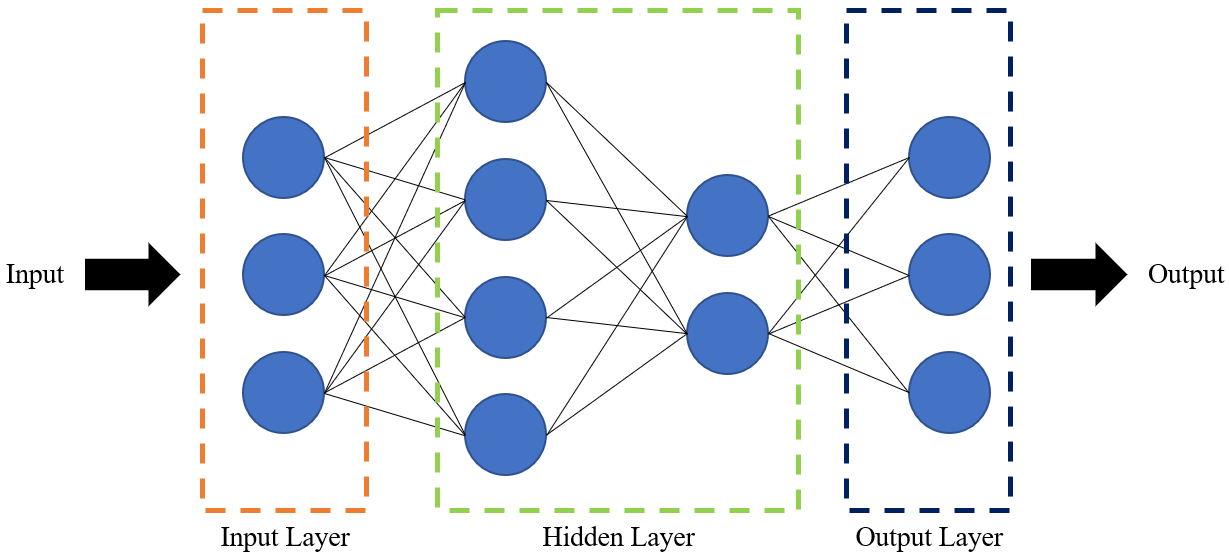
\includegraphics[width=0.6\textwidth]{Figures/Application To Deep Learning/DNNarch.png}
  \caption{Model of fully-connected (feed-forward) \acrshort{dnn}}
  \label{fig:DNNarch}
\end{figure}

\subsection{DNN Architectures}

Current \acrshort{dnn} architectures are grouped into three types of architecture, depending on the fundamental primitive operation being performed. These are Convolutional Neural Networks (\acrshort{cnn}), Recurrent Neural Networks (\acrshort{rnn}) and Unsupervised Pretrained Networks (\acrshort{upt}). 

\subsubsection{Convolutional Neural Networks (CNN)}
Convolutional Neural Networks can extract features from data via the convolution operation, being mainly used for image and object recognition and sound analysis. This type of architecture excels when there is some structure in the input data, that is, the data contains sets of specific patterns, organized in a spatial manner, that the neural network can learn to recognize.

The \acrshort{cnn} architecture generally follows the following pattern: input layer, feature-extraction layers and classification layer. The input layer receives a form of three-dimensional data, usually an image with a specific height and width and a depth value (representing color or intensity). The feature extraction layers perform higher-order features extract from the input, generally by performing patterns of convolution layers and pooling layers. Finally, the classification layer is a vector of size \textit{N}, where each output represents a score of prediction confidence for the input to be of a given output class.

Three common datasets used to compare and analyse the \acrshort{cnn}  performance are MNIST~\cite{lecun_yann_and_cortes_corinna_mnist_1999}, CIFAR~ 10~\cite{krizhevsky_learning_2009} and ImageNet~\cite{deng_imagenet_2009}, each with increased input complexity, number output classes and overall dataset size. MNIST consists of 70 000 images of handwritten digits 0 to 9, CIFAR10 consists of 60 000 images organized of 10 object and animal classes, and ImageNet is a collection of 14 million images of 20 thousand different classes. 

\subsubsection{Recurrent Neural Networks (RNN)}

Recurrent Neural Networks have the added capability of sending information over time-steps. This characteristic allows this type of architecture to have parallel and sequential data modeling, not only recognizing features from each input but also allowing for the extraction of features from the sequences of inputs, modeling the time dimension. 

acrshort{rnn}s are used to model time-series, language, audio, and text since this type of data is inherently ordered and context-sensitive. acrshort{rnn}s contain feedback loops between the layers, in order for each layer to have insights about what comed before. The model prediction follows the general format presented in Equation \ref{eq:rnn}, where $y$ represents the model prediction and $x$ the model inputs. The equation reflects the influence of previous inputs for each output.
\begin{equation}
    \label{eq:rnn}
    y[n] = x[n] + ... + x[n-i]
\end{equation}

The primitive that compose the feature extraction of \acrshort{rnn} models are LSTM - Long Short Term Memory. This type of layer unit has three gates - input, output and forget gates. The content of each LSTM is moduled by the input and forget gates; this change reflects on the value stored at the memory cell. If both gates are closed, the memory content remains unmodified between the current time-step and the following. The LSTM structure allows for information to be retained/forgotten on the memory cell across different time-steps.


\subsubsection{Unsupervised Pre-trained Networks (UPN)}
Unsupervised Pretrained Networks is a category of \acrshort{dnn} architectures that encompasses architectures such as autoencoders and generative adversarial networks (\acrshort{gan}s). This class of \acrshort{dnn} architecture departs from the previous ones, by learning in an unsupervised manner, meaning that the input data given to the network is not previously labeled. This introduces an extra degree of learning freedom by allowing the network to identify and recognize patterns that distinguish the output classes the most.

Autoencoders are used to learn efficient data codings and can be applied for dimensionality reduction or augmentation. Autoencoders allow for the reduction of noise in a signal or to perform a resolution increase on an image. \acrshort{gan}s can be used to perform sound and video synthesis from images or text using two neural networks in parallel - a discriminator and a generative network. First, the generative network creates a synthesized output from the given input given. Then the discriminator network tries to classify the input as real or synthesized, providing the classification to the generative network. With this data loop, the generative network updates their weights to fit best what is described as real data.


\subsection{Training and Inference}

The mathematical description of the \acrshort{dnn} training process, (see Equation \ref{eq:loss}), is equivalent to treating the network as a loss function $L$, where inputs $X$, outputs $Y$ and the network's parameters weights - $W$ and bias $b$ are function arguments. The training session's objective is to optimize the in-network parameters  $W$ (weights) and $b$ (bias) to minimize the overall loss.

\begin{equation}
    \label{eq:loss}
    (W,b) = \arg\min_{W} L(X,Y,W,b)
\end{equation}

The \acrshort{dnn} training is an iterative process, where at the end of each iteration, a loss value is computed, and the set of in-network parameters is updated. This loss value represents how well are the input parameters being modeled by the network. As the number of training iterations increases, the loss value reduces and converges to a minimum, at which the model accuracy prediction will be at its maximum. At this point, the training session can be stopped.

The most common method for the parameters update is the Stochastic Gradient Descent (\acrshort{sgd}) algorithm (see Equation \ref{eq:update}), an iterative algorithm that, after processing mini-batches of the training data, computes new weights and bias for each neuron. 

\begin{equation}
    \label{eq:update}
    W_{i+1} \xleftarrow{} W_i - \alpha \sum_{n=1}^{m}\frac{\partial L}{\partial W_i}
\end{equation}

In Equation \ref{eq:update}, $m$ represents the number of mini-batches to run, $W_i$ is the current parameter, $W_{i+1}$ the update parameter, $\alpha$ the learning rate and $\frac{\partial L}{\partial W_i}$ the partial derivative of the loss function $L$ in order to the parameters. This last equation is obtained by applying the derivative chain rule in a backward-cascade fashion with respect to inputs, outputs, and parameters of each \acrshort{dnn} layer.

Each iteration of the training process is composed of a forward and backward data propagation. On the forward propagation, the loss function for the current in-network parameters is evaluated, computing the loss value. By performing the backward propagation, the partial derivative $\frac{\partial L}{\partial W_i}$ of each of the parameters is obtained to apply the \acrshort{dnn} algorithm . 

The inference (or prediction) process corresponds to performing a forward propagation, with the intended input, on a previously trained neural network. At the output layer, a set of values (or probabilities) is computed, corresponding to the model's prediction to the given inputs.

\subsection{High-Level Libraries and Software Frameworks}

The popularization of \acrshort{gpu}s as the defacto \acrshort{dnn}s execution device comes at the cost of the availability of high-level libraries and frameworks from device manufacturers and other software houses. The available \acrshort{gpu} libraries implement the underlying mathematical operations performed during the \acrshort{dnn}s, while the frameworks operate on the execution of \acrshort{dnn}s by masking the complexity of creating, training and using these models~\cite{jain_performance_2019}.

The most used libraries are cuBLAS\footnote{developer.nvidia.com/cublas} and cuDNN\footnote{developer.nvidia.com/cudnn}, by NVIDIA and rocBLAS\footnote{github.com/ROCmSoftwarePlatform/rocBLAS} and MIOpen\footnote{github.com/ROCmSoftwarePlatform/MIOpen}, by AMD that implement the most optimize versions of matrix multiplication, convolution, and other kinds of mathematical operations to be used on the \acrshort{dnn} models. For the frameworks, TensorFlow\footnote{tensorflow.org/} and PyTorch\footnote{pytorch.org/} are open-source frameworks developed by Google and Facebook, respectively that allow for easy implementation of the models in \acrshort{gpu}s.

%%%%%%%%%%%%%%%%%%%%%%%%%%%%%%%%%%%%%%%%%%%%%%%%%%%%%%%%%%%%%%%%%%%%%%%%
\section{DNN Performance and Energy Efficiency Improvement}
\label{section:DNN_conventional}

\acrshort{dnn} are usually characterized by significant computational burdens, particularly when considering the training of very deep and complex networks that deal with high dimensional data, such as images and videos. For such purpose, researchers (and data scientists, in general) often rely on accelerators, such as \acrshort{gpu}, to cope with the associated computational burden and reduce the training time. As a result, \acrshort{gpu} are now commonly deployed on most supercomputers, data centers and other computational infrastructures related to the development of artificial intelligence algorithms.

Additionally, several software frameworks, algorithms and techniques have been proposed to manage and optimize the execution of  \acrshort{dnn} on \acrshort{gpu} (e.g., Mittal~\cite{mittal_survey_2019}). However, most optimization techniques neglect the training phase's energy impact, usually resulting in considerable costs. 

To overcome this problem, researchers have also explored other solutions that allow mitigating the energy impact of neural network training. One particular and common approach relies on the use of low-precision arithmetic (e.g., Nabavinejad~\cite{nabavinejad_coordinated_2019}), eventually trading network accuracy with increased processing performance and lower energy consumption.

Researchers have also looked at alternative approaches, such as exploiting \acrshort{dvfs} on both the inference and training phases. In fact, by carefully selecting the used voltage-frequency (V-F) levels, significant energy savings can be obtained, although depending on the considered \acrshort{dnn} architecture and computing  device~\cite{tang_impact_2019}. This is achieved by a careful balance between the performance and power consumption of the different \acrshort{gpu} components  (particularly the core and global memory) to minimize stalls in the compute cores. In fact, not only can \acrshort{dvfs} be used to decrease the power consumption, but it can also boost the system performance~\cite{tang_impact_2019}, by increasing the voltage and frequency levels (as long as the GPU total power envelope and thermal limits are not surpassed).

%Nevertheless, as discussed, most state-of-the-art works only consider tightly coupled V-F levels, which are often predefined by GPU manufacturers and neglect the voltage margin that is usually introduced to guarantee fail-safe designs well as its variation with the kernel instruction sequence and the corresponding use of specific \acrshort{gpu} components. 


Supported on the performed \acrshort{gpu} characterization to non-conventional V-F pairs, this work continues by exploring the impact of these configurations on the \acrshort{cnn}s layers and training and inference.

%%%%%%%%%%%%%%%%%%%%%%%%%%%%%%%%%%%%%%%%%%%%%%%%%%%%%%%%%%%%%%%%%%%%%%%%
\section{Non-conventional V-F on CNNs}
\label{section:baseline}

As it was referred in Section~\ref{sec:under_int_app}, Tang~\cite{tang_impact_2019} has recently studied the impact of frequency scaling on the performance and energy consumption of \acrshort{dnn} executed in \acrshort{gpu}. By extending this study with the capability to also apply undervoltage techniques, a broader range of \acrshort{dvfs} configurations are herein envisaged to provide even greater benefits. 

Another important characteristic of \acrshort{dnn} is their tolerance to a certain degree of computation errors \cite{zhang_approxann_2015}, without any significant change in the training and inference results. Consequently, it is crucial to complement the characterization performed in the Chapter~\ref{chapter:gpu_char} with the voltage scaling effects in \acrshort{dnn} training and inference phases and, in particular, with its influence on the computation errors that might occur when exploring the existing voltage margins.

As discussed, at the particular case of the \acrshort{cnn}, its feature extraction ability is supported by the convolution operator. Nonetheless, \acrshort{cnn} also includes other types of layers, such as fully connected and pooling layers. However, convolution and fully connected layers take up to $97\%$ of the \acrshort{gpu} energy consumption~\cite{li_evaluating_2016}, which makes them particularly suited to exploit energy-saving mechanisms. 

Hence, to assess and apply non-conventional V-F pairs on the execution of \acrshort{cnn}s, the high-level deep learning framework PyTorch and the default mathematical libraries (rocBLAS and MIOpen) provided by the considered \acrshort{gpu} manufacturer (AMD) were extensively evaluated. This section reports the main achieved conclusions for the convolution operator and fully connected layers.

\subsection{Convolution Layer}

The MIOpen library provides multiple convolution implementations, being the \textit{Direct}, \textit{GEMM} and \textit{Winograd}~\cite{khan_miopen_2019} the ones that are more often used. 
At the beginning of the execution, this library performs one convolution operation with each of the algorithms that are able to solve the given convolution. Then, the algorithm that takes the shortest execution time is chosen and used to perform the remaining convolutions of the current layer. The convolution layer is defined by the parameters presented in Table~\ref{tab:convparams}. 

\begin{table}[htbp]
\caption{Convolution Parameters}
\begin{center}
\begin{tabular}{cl}
\hline
\textbf{Parameter}&\textbf{Description} \\ 
\hline
W, H & Input Width, Height\\
N & Mini-batch Size \\
C, K & Number of features, kernels \\
R, S & Kernel Width,Height\\
Pad\_W, Pad\_H & Padding Width, Height \\
Str\_W, Str\_H & Stride Width, Height \\
\hline
\end{tabular}
\label{tab:convparams}
\end{center}
\end{table}

A valid claim to be made is that if there is a convolution algorithm that is more energy-efficient than the others, and so, of particular interest for the work. One of the input parameters of the convolution \acrshort{api} is the algorithm selection that disables the automatic algorithm selection. 
The execution time, and energy and power consumption of all algorithms were measured while executing 100 different convolutions layer configurations from the DeepBench benchmark\footnote{github.com/baidu-research/DeepBench}, with each algorithm being executed ten times with the median results being taken. The result showed that the algorithm that achieved the shortest execution time in all cases also achieved the best energy consumption. By looking at the power consumption across the different algorithms, the result showed that it was similar in all cases. Two other important results were that no algorithm proved to be the fastest for all or subset of configurations and that not all convolution layer configurations are able to be mapped on the pre-compiled and optimized kernels, that implement the different algorithms, available in the library. The results show that even though the technique of measuring the execution time at the beginning of the execution appears simplistic and with space to be optimized, in reality, that is not the case. Measuring the execution time at the beginning of the execution for all possible execution ways optimizes both the performance as well as energy consumption. This technique also brings the benefit of optimizing the execution to the current \acrshort{gpu} state and utilization, which is one of the premisses of the presented work.

To conduct the convolution analysis, a set of 20 distinct convolution layer configurations was selected from the DeepBench benchmark to understand how each algorithm is affected by V-F configuration, both in its inference and training phases.



\subsubsection{Layer Guardband and Characterization}

Figure~\ref{fig:Convolution_guardband} presents the set of valid voltage ranges that were obtained for the inference and training phases of the convolution layer. Comparing these results with those obtained in the individual component characterization, it can be observed that some computation errors (and even some \acrshort{gpu} crashes) were detected at lower frequencies. In fact, since this operation is more complex and requires the utilization of multiple architectural components, the undervoltage limit is more likely to be violated by the voltage drops induced by the activation and deactivation of the \acrshort{gpu}  architectural components \cite{thomas_core_2016}. This phenomenon will make certain parts of the \acrshort{gpu} not to work properly (even momentarily), producing an increased rate of computation errors and an increased crash threshold voltage. 


\begin{figure}[htbp]
    \centering
        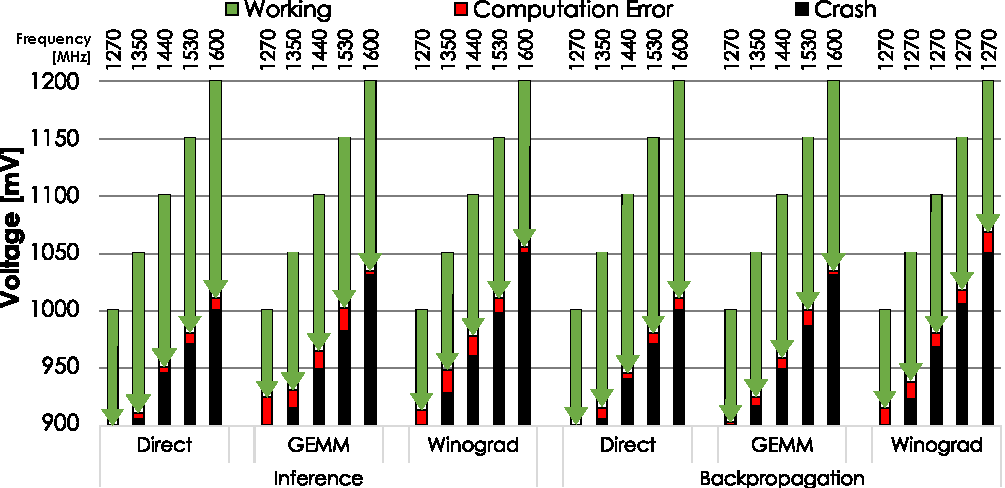
\includegraphics[width=0.75\textwidth]{Figures/Application To Deep Learning/Convolution_Guardband.pdf}
        \caption{Core Domain - Convolution Layer - Usable voltage range.}
    \label{fig:Convolution_guardband}
\end{figure}

When comparing the three convolution algorithms, it is observed that \textit{Direct} allows for the greatest amount of undervoltage, followed by \textit{GEMM} and \textit{Winograd}. The \textit{Direct} algorithm is the simpler of the three, with no data transformation and movement being necessary for its execution. In contrast, \textit{GEMM} and \textit{Winograd} need some data pre-processing before the convolution is performed. This extra step relies on the activation of more \acrshort{gpu} components, making these algorithms more prone to induce voltage drops. 

When comparing the training and inference phases, it is observed that they present similar undervoltage capabilities (for all algorithms), with the crash point diverging only around $10$mV. However, the training algorithm is more prone to the introduction of computation errors, starting to be observed at a lower degree of undervoltage when compared to the inference.

Figures~\ref{fig:Convolution_behaviour} and \ref{fig:Convolution_EDP} illustrates the impact of non-conventional V-F on energy consumption, execution time and \acrshort{edp}. When working with the default voltage level of each frequency (dashed lines), the \textit{Direct} and \textit{GEMM} algorithms exhibit a valley in their performance chart, with the frequency of $1530$~MHz providing the best performance. In contrast, the \textit{Winograd} achieves its best performance with the lowest frequencies. Upon the introduction of independent voltage scaling, it is possible to improve the execution time and energy consumption (in comparison with the default voltage) by $8\%$ and $23\%$, $19\%$ and $8\%$, and $14\%$ and $24\%$ for the \textit{Direct}, \textit{GEMM} and \textit{Winograd} algorithms, respectively. 

\begin{figure}[htb]
  \begin{subfigmatrix}{2}
    \subfigure[Inference]{\label{fig:Convolution_Inference_behaviour}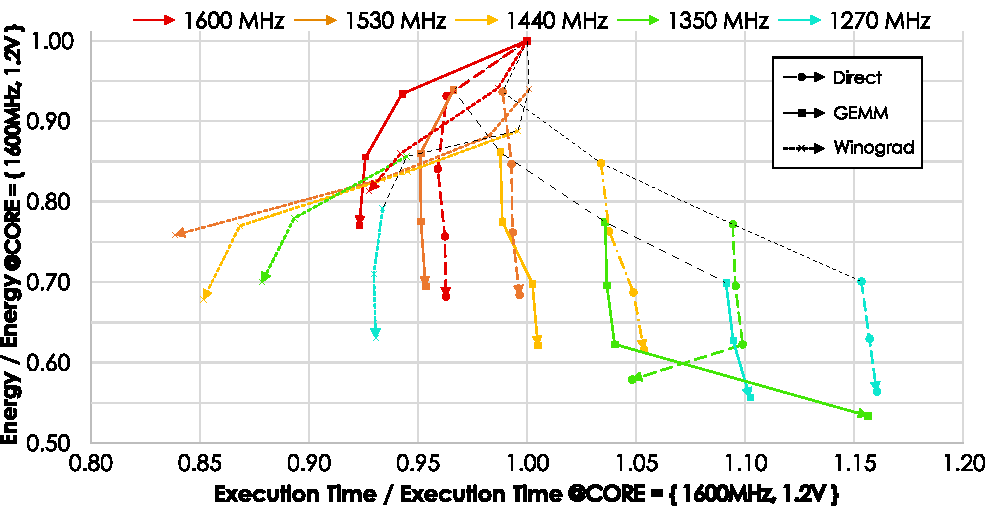
\includegraphics[width=0.75\textwidth]{Figures/Application To Deep Learning/Convolution_Inference_Behaviour.pdf}}
    \subfigure[Training]{\label{fig:Convolution_Backprop_behaviour}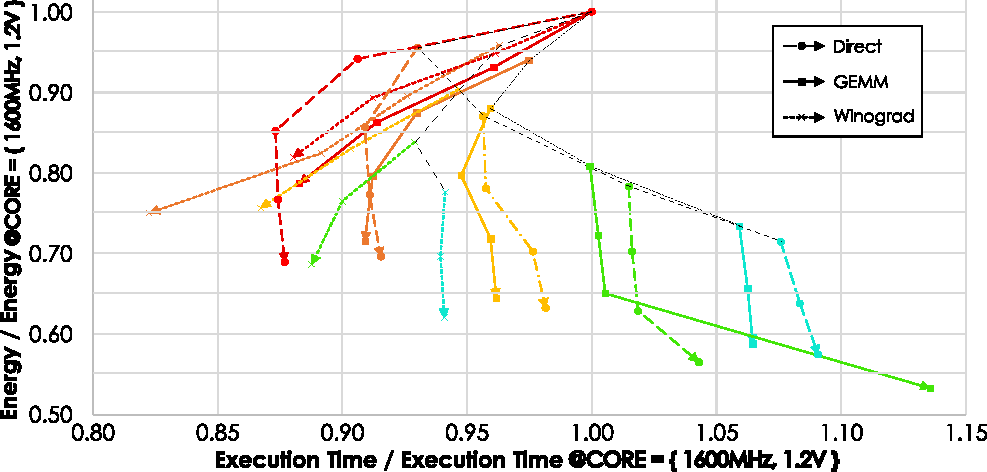
\includegraphics[width=0.75\textwidth]{Figures/Application To Deep Learning/Convolution_Backprop_Behaviour.pdf}}
  \end{subfigmatrix}
  \caption{Core domain - .}
  \label{fig:Convolution_behaviour}
\end{figure}

The \acrshort{edp} charts depicted in Figure~\ref{fig:Convolution_EDP} indicates that the most energy-efficient configuration for the three algorithms is at the lowest frequencies and maximum undervoltage possible. At these configurations, although the execution time is reduced by $16\%$ (for the \textit{Direct} and \textit{GEMM} algorithms), it is still possible to achieve a reduction in energy consumption of up to $46\%$. The use of the most efficient configuration for the \textit{Winograd} algorithm improves both the execution time and the energy by $15\%$ and $32\%$, respectively.

\begin{figure}[htbp]
    \centering
        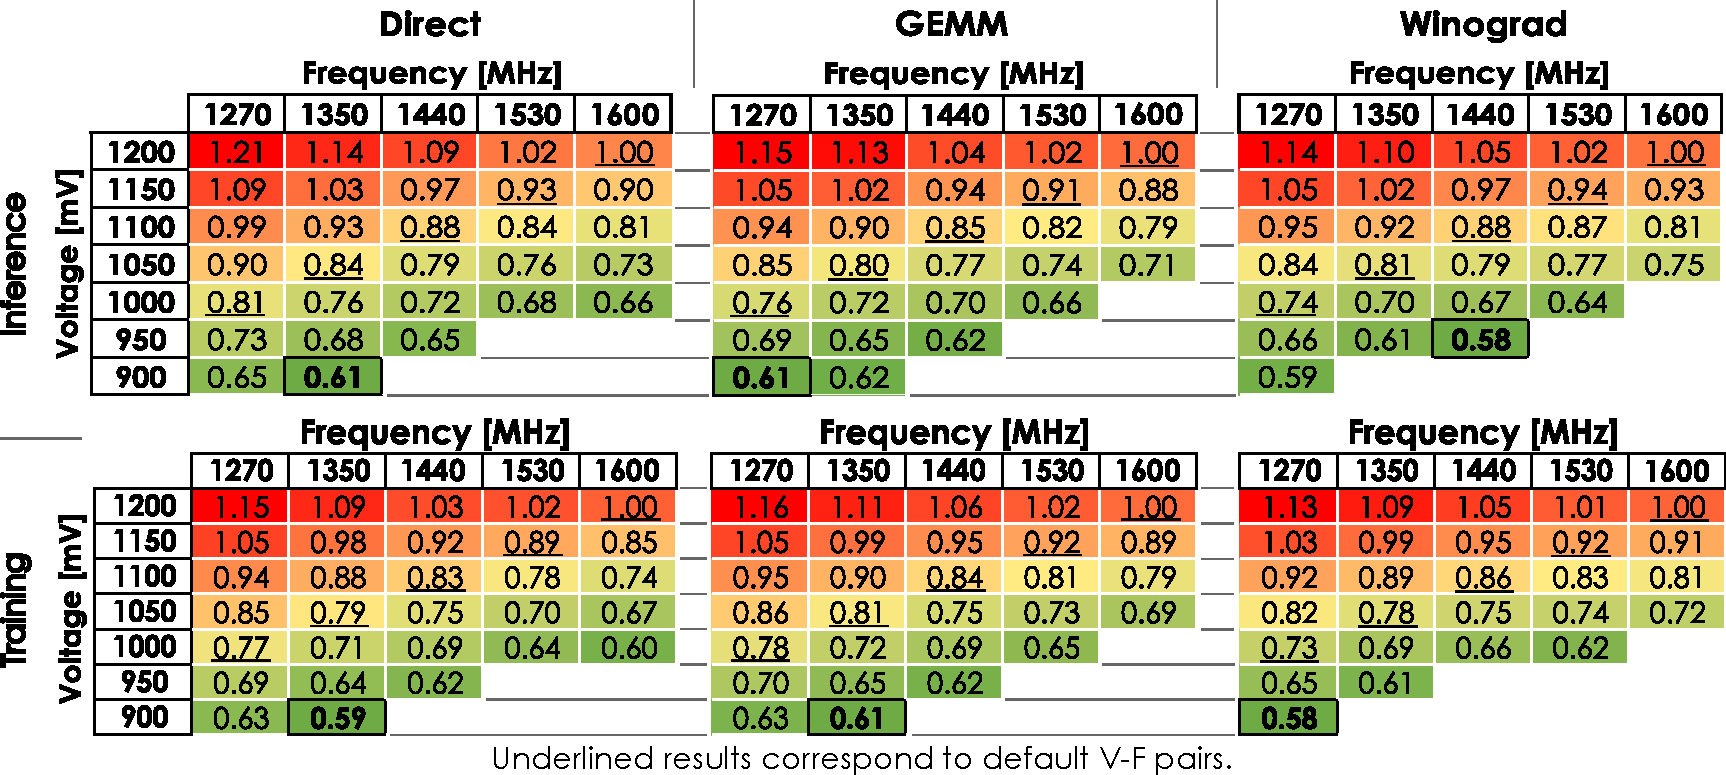
\includegraphics[width=1.0\textwidth]{Figures/Application To Deep Learning/Convolution_EDP.pdf}
        \caption{Core Domain - Convolution Layer - EDP heatmap for the three algorithms.}
    \label{fig:Convolution_EDP}
\end{figure}



\subsection{Fully-Connected Layer}


The RocBlas library provides a single API for matrix multiplication, the underlying mathematical operation of the fully connected layer. By analyzing the performance counters and the kernels called by the library, it is possible to understand that multiplication is performed in one of two ways depending on the size of the matrices.
According to to~\cite{dutot_high-performance_2016}, small matrices are first loaded to Cache, and all the operations are performed with the data in this component, making the operation compute bounded. For large matrices, the matrix multiplication is split, performing the multiplication in a tilling fashion. In this way, submatrices are loaded to the local caches, and the submatrices of results are produced. When the submatrix is consumed, another pair is loaded, and the process repeats until the full computation is performed. The threshold size corresponds to the size of the L1 Cache. 


\subsubsection{Layer Characterization}

Non-conventional V-F will impact the two implementations of the matrix multiplication in different ways. For small matrices, 
since before the computations start, all the necessary data is already available on the local caches, 
it is the ALU that will limit the undervoltage. Consequently, it is expected that a valley-like shape is observable in the performance chart after the application of frequency scaling (see section~\ref{sec:MAC_behaviour}). On the other hand, for large matrix sizes, the Cache will be stressed the most, with constant requests on the DRAM-Cache controller limiting the undervoltage. Consequently, the results will be similar to those that were observed in section~\ref{sec:cache_guardband} and \ref{sec:cache_sm__behaviour}. Figure~\ref{fig:MatrixMult_guardband} illustrates the results of the experiment and confirms the prediction: for small matrix sizes, it is possible to perform a higher degree of undervoltage. 


\begin{figure}[htbp]
    \centering
        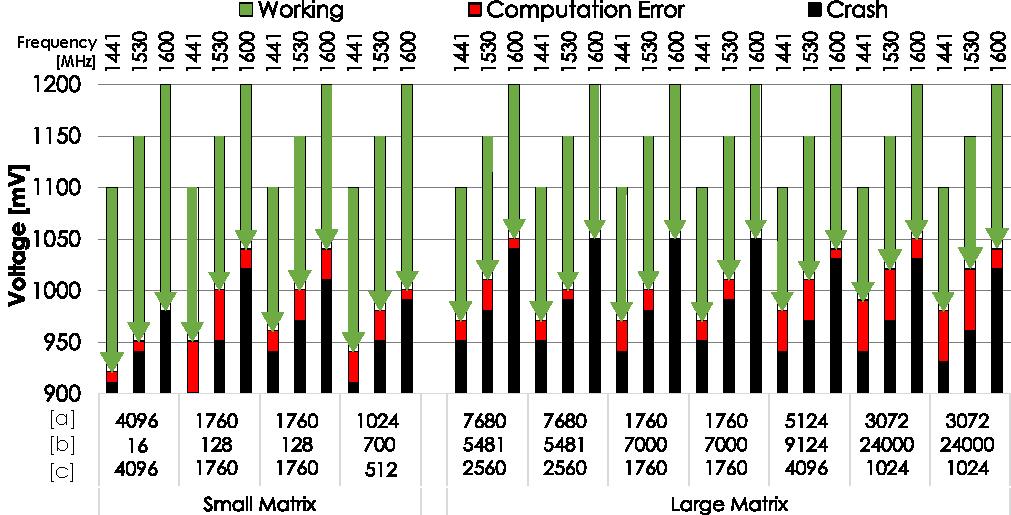
\includegraphics[width=0.75\textwidth]{Figures/Application To Deep Learning/MatrixMul_guardband.pdf}
        \caption{Core Domain - Fully-Connected Layer - Usable GPU core voltage range. Values represent matrix sizes, example $A_{a \times b} \cdot B_{b \times c}$.}
    \label{fig:MatrixMult_guardband}
\end{figure}


Figures~\ref{fig:MatrixMult_behaviour} and \ref{fig:MatrixMult_EDP} present that it is possible to have an improvement in the execution time and energy consumption for both types of computations. The EDP chart indicates the same energy efficiency configuration for both cases, which results in an average reduction of $52\%$ in energy consumption and $8\%$ of improvement of the execution time.


\begin{figure}[htbp]
    \centering
        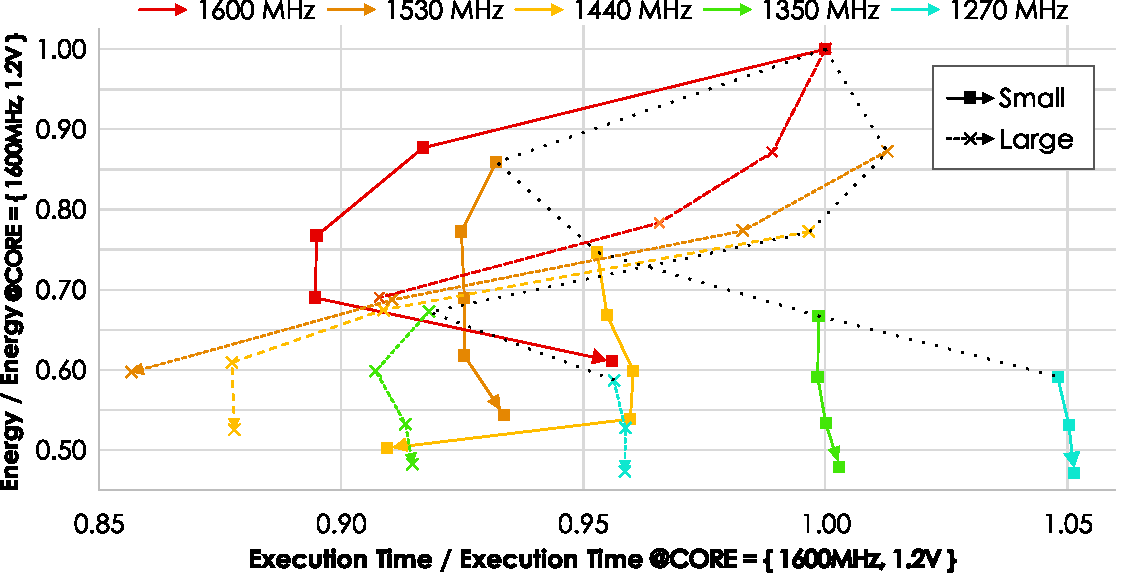
\includegraphics[width=0.75\textwidth]{Figures/Application To Deep Learning/MatrixMul_behaviour.pdf}
        \caption{Core Domain - Fully-Connected Layer - Behaviour.}
    \label{fig:MatrixMult_behaviour}
\end{figure}





\begin{figure}[htbp]
    \centering
        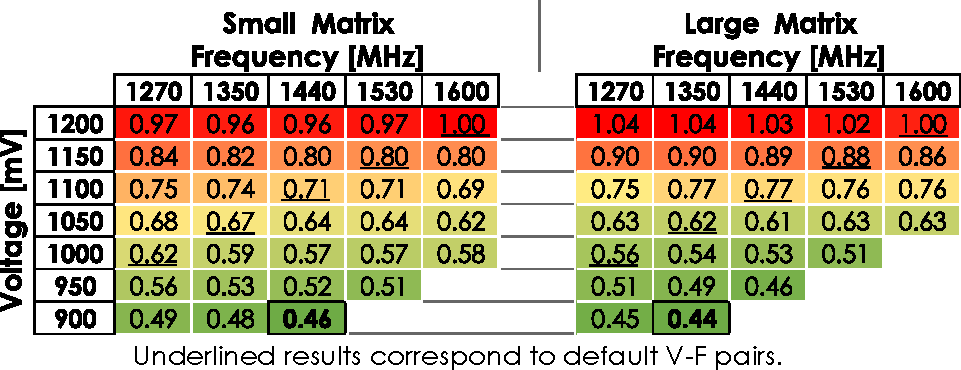
\includegraphics[width=0.75\textwidth]{Figures/Application To Deep Learning/MatrixMul_EDP.pdf}
        \caption{Core Domain - Convolution Layer - .}
    \label{fig:MatrixMult_EDP}
\end{figure}

\subsection{Error Analysis}

To evaluate the occurrence of computation errors due to the utilization of non-conventional V-F scaling, each benchmark was executed with the default "automatic'' parameterization and the V-F pair under testing with the same input data. A \textit{warmup\_kernel} was also executed before each of these two runs, to fill the cache with random data. 


For the error analysis of the \acrshort{cnn} layers, a different error metric was adopted due to the utilization of software libraries (versus custom kernels) operating over floating-point numbers (as before, generated from an uniform distribution in the interval $[0.1~;~1]$ to ensure that operations are never applied to numbers with significantly different exponent values). These libraries can launch the kernels in a different order, changing the order of operations, with a possible impact in the final result. In fact, by conducting experiments on the default voltage, it was observed that the order of kernel execution resulted in a relative output difference not greater than $10^{-6}$. In accordance, a computation error was asserted whenever the relative difference in each position of the output vectors was greater than or equal to  $10^{-5}$.

\subsubsection{Convolution Layer}

Figure~\ref{fig:Convolution_errors} depicts the distribution of the output results of the convolution layer for the three considered convolution algorithms (at both inference and training phases) for the minimum usable voltage values (i.e., before \acrshort{gpu} crash) across all considered core frequency values. The obtained results emphasize the little effect of the applied undervoltage on the computed values. Most of the output results are still almost entirely accurate, and only a small portion of the results present deviations. In fact, it should be emphasized that not only is the fraction of non-accurate results very small, but the normalized relative error of those non-accurate results has a shallow magnitude. A particular observation is worth noting about the results of the inference phase with the \textit{GEMM} algorithm. Although the amount of non-accurate results is greater than in the other configurations, the normalized relative error's magnitude is much smaller.

\begin{figure}[htbp]
    \centering
        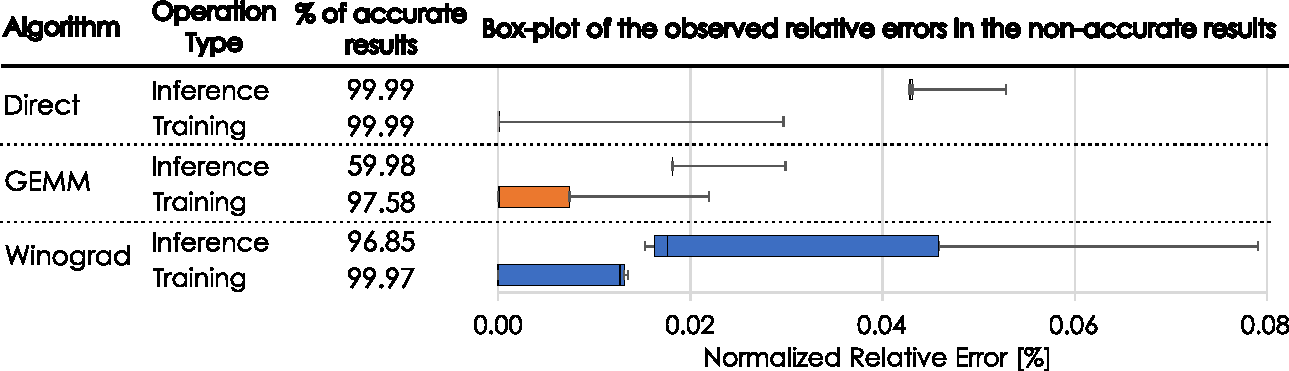
\includegraphics[width=0.8\textwidth]{Figures/Application To Deep Learning/Convolution_Error_Distribution.pdf}
        \caption{Convolution Layer - Average percentage of accurate results and relative error distribution of non-accurate outputs for the minimum usable core voltage across all considered core frequency values.}
    \label{fig:Convolution_errors}
\end{figure}



\subsubsection{Fully Connected}

Figure~\ref{fig:MatrixMult_errors} represents the same evaluation for the Fully Connected Layer, for both small and large matrices. Even at these extreme configurations, it is observed that most results are still computed with full accuracy (98\% of the cases), with a normalized relative error as low as $1.37\times10^{-3}$ (on the remaining $2$\% of the cases).

\begin{figure}[htbp]
    \centering
        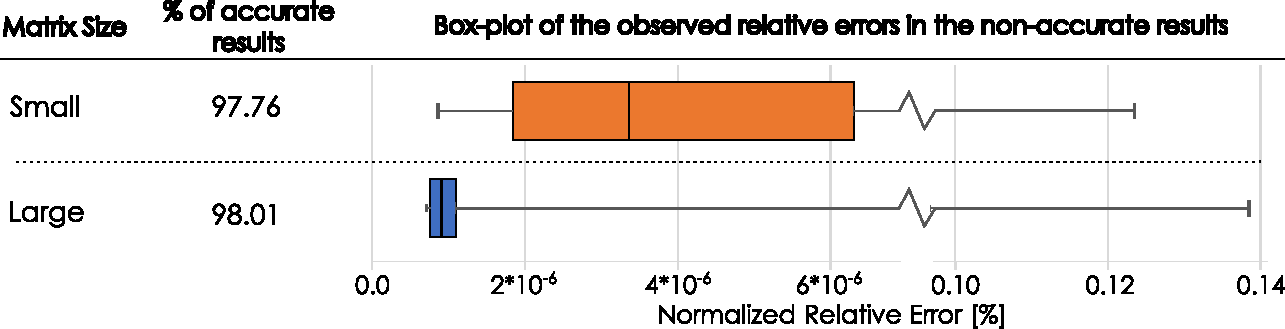
\includegraphics[width=0.8\textwidth]{Figures/Application To Deep Learning/MatrixMul_Error_Distribution.pdf}
        \caption{Fully Connected - Average percentage of accurate results and relative error distribution of non-accurate outputs for the minimum usable core voltage across all considered core frequency values.}
    \label{fig:MatrixMult_errors}
\end{figure}

Hence, the obtained results demonstrate that the amount of error introduced by these lowest voltages before crash conditions, on the two most important layers, are cooped with both \acrshort{dnn} training and inference, demonstrating the ample viability of this approach.


%%%%%%%%%%%%%%%%%%%%%%%%%%%%%%%%%%%%%%%%%%%%%%%%%%%%%%%%%%%%%%%%%%%%%%%%
\section{CNN training and inference with non-conventional V-F}
\label{section:enhanced}

The preliminary assessment of the \acrshort{cnn} primitives exhibits the same behavior of the primitive operations analyze, performed on the Chapter~\ref{chapter:gpu_char}. It is possible to safely undervolt the \acrshort{gpu} of the two main \acrshort{cnn} primitives without compromising the accuracy and with energy and performance gains. With so, the logical next step is to adapt the optimization mechanism described on Chapter~\ref{chapter:mech} to the training of complete state-of-the-art \acrshort{cnn}s.


This section starts by presenting the usability of non-conventional V-F on the complete training of \acrshort{cnn}s, followed by how the optimization mechanism was adapted to achieve the same energy efficiency gains automatically.

\subsection{Feasibility Assessment}

The results that were obtained in the previous section evidence that the small number and relative amount of computation errors introduced by these near threshold conditions is well cooped with the operations that are conducted in \acrshort{dnn} layers. However, the same evaluation urged to be done for the whole network.


Following the same methodology as before, an exploration of the frequency and voltage was performed for the training + inference and inference phase of four complete well-know \acrshort{cnn} models. The tested models are LeNet, VGG11, AlexNet and WideResNet, corresponding to increasing model size, complexity, and characteristics. The feasibility assessment will prove that using such configurations is allowed by the algorithms under execution, both with negligent impacts on the models' final training accuracy and with energy-efficiency improvements. To guarantee that the changing V-F is the only source of the observed variation, in all tests, the networks' weights are initialized with the same value.


\subsubsection{Training and Inference}

Table~\ref{tab:trainingAcc} presents the median classification accuracy over ten training runs and demonstrates that, when compared with the default setup (i.e., undervolt = 0), the introduced computation errors do not induce any significant change in the network's final training accuracy. 
In more detail, Figure~\ref{fig:CNN_loss}, presents the behavior of the loss and model accuracy measured on the test set over the training session. It is possible to observe that the two metrics' progress is, within small variations, the same for all tested V-F configurations.

\begin{table}[htb]
    \centering
    \caption{Comparing CNN training test set accuracy with the application of different undervoltage levels.}
    \label{tab:trainingAcc}
    \begin{tabular}{rcccc}
        \multicolumn{1}{l}{{\textbf{Amount of undervolt {[}mV{]}}}} &
          \textbf{AlexNet {[}\%{]}} &
          \textbf{LeNet {[}\%{]}} &
          \textbf{VGG11 {[}\%{]}} &
          \textbf{WideResNet {[}\%{]}} \\ \hline
        \textbf{0}   & 76.59 & 59.84 & 86.14 & 80.32 \\
        \textbf{50}  & 76.48 & 60.08 & 86.14 & 80.39 \\
        \textbf{100} & 76.60 & 59.94 & 86.04 & 80.23 \\
        \textbf{150} & 76.61 & 60.12 & 86.39 & 80.08 \\ \hline
        \multicolumn{1}{l}{{\textbf{Number of trained epochs}}} &
          50 &
          100 &
          30 &
          30
    \end{tabular}%
    
\end{table}


\begin{figure}[htb]
    \centering
        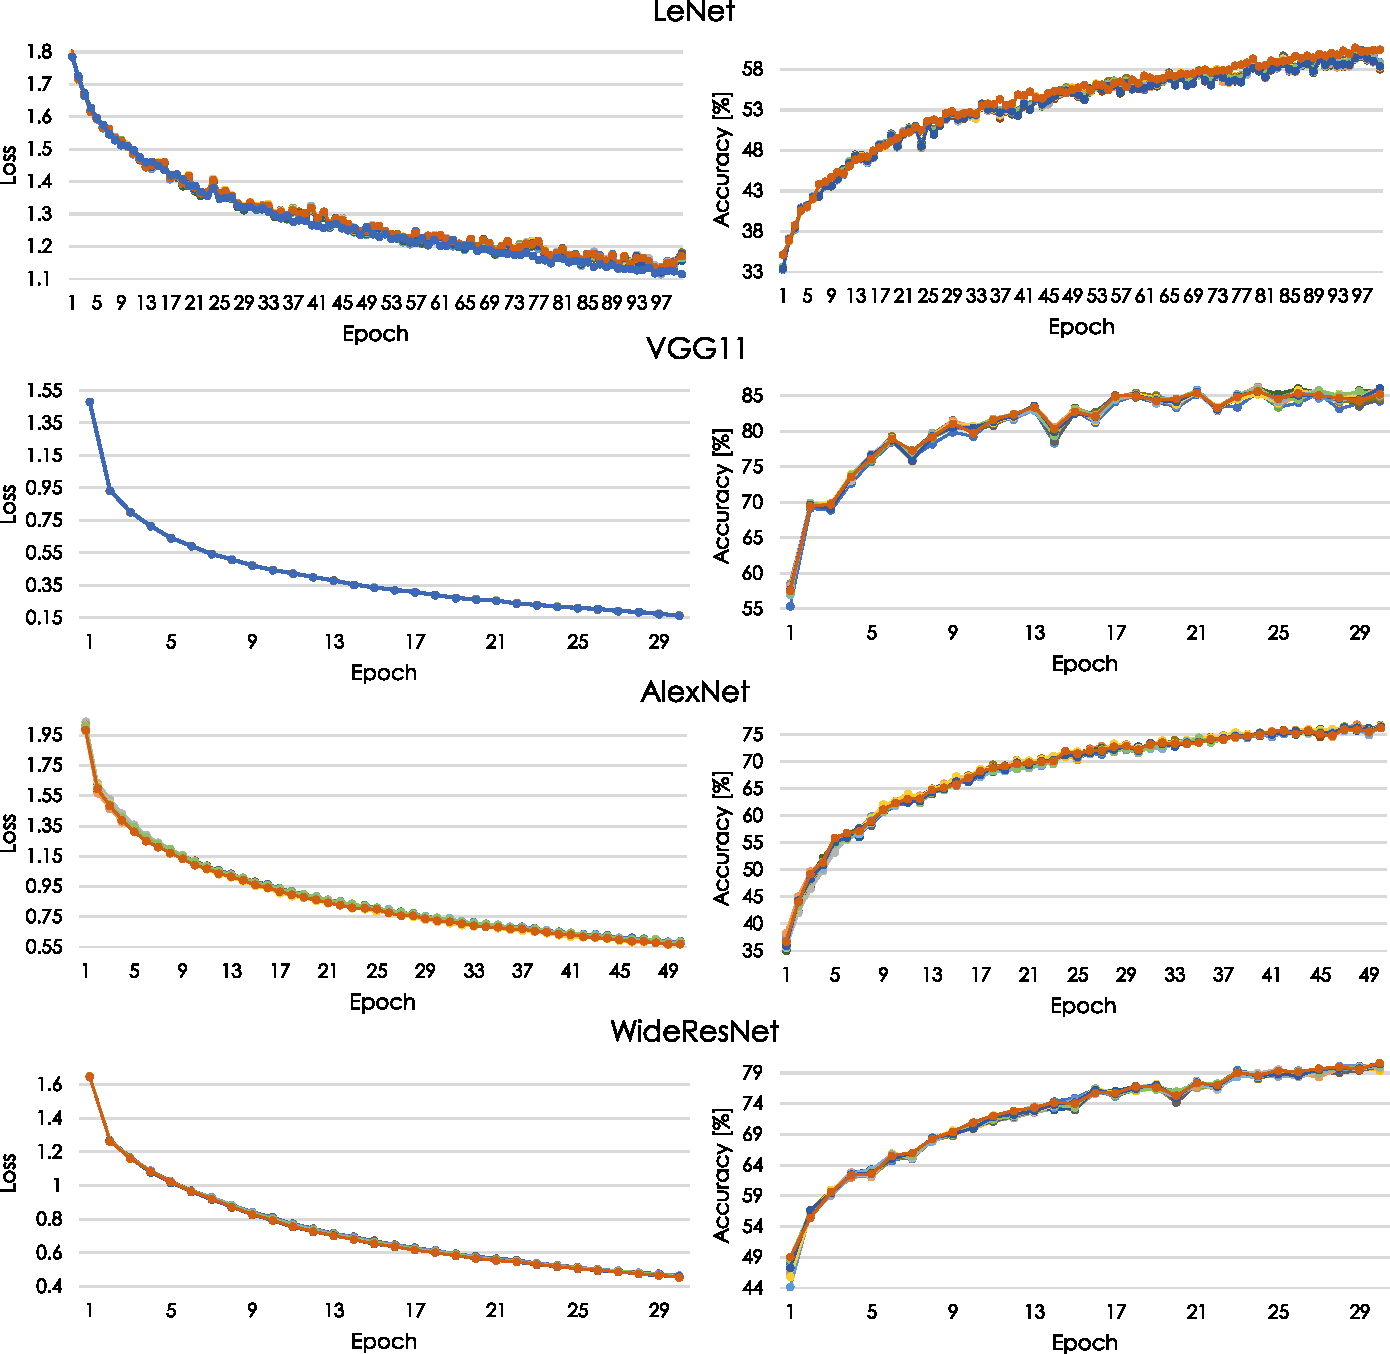
\includegraphics[width=0.8\textwidth]{Figures/Application To Deep Learning/CNN_loss_acc.pdf}
        \caption{Core domain - CNN models - superposition of all V-F configuration test set loss and model accuracy.}
    \label{fig:CNN_loss}
\end{figure}

\begin{figure}[htb]
    \centering
        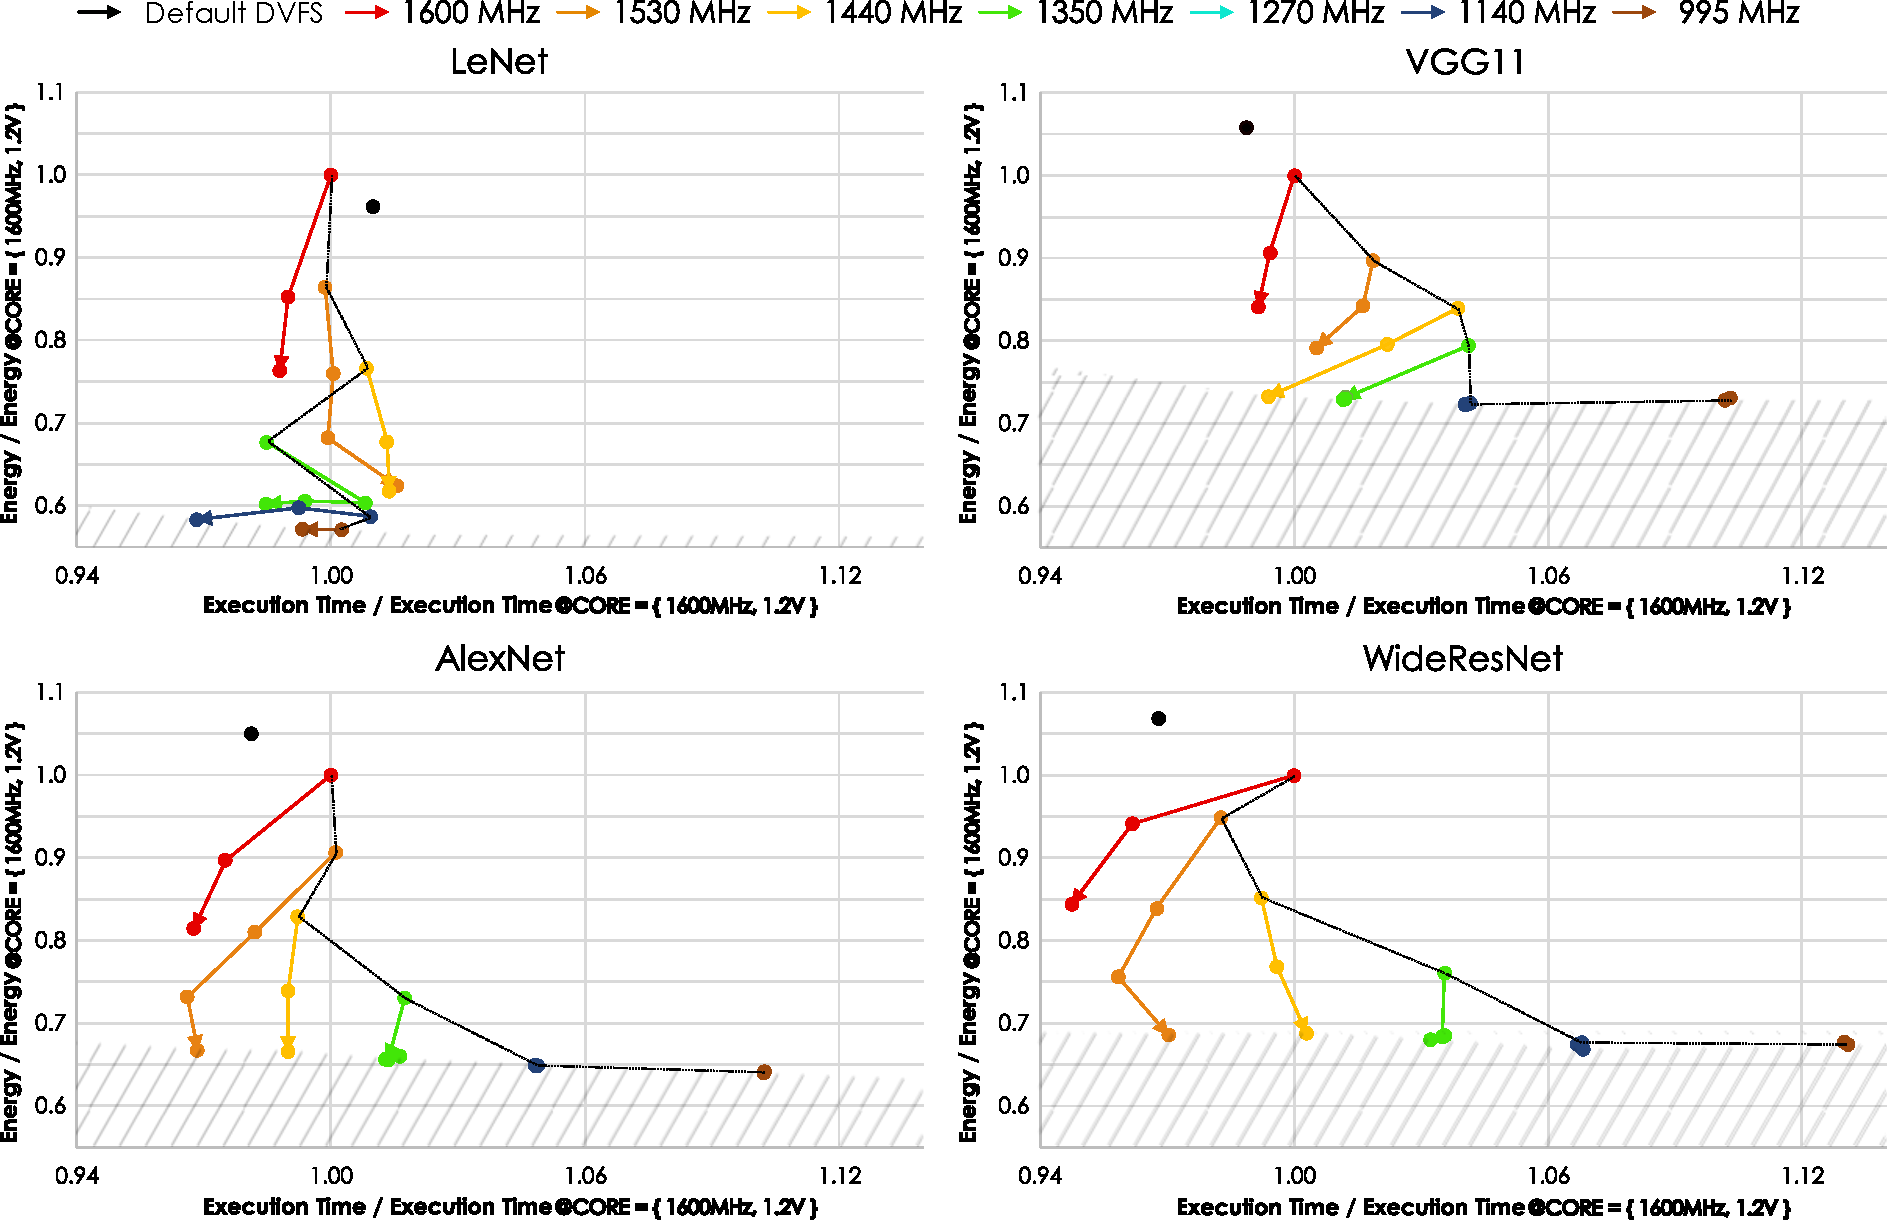
\includegraphics[width=0.8\textwidth]{Figures/Application To Deep Learning/CNN_behaviour.pdf}
        \caption{Core domain - CNN models - Normalized energy consumption and execution time for training + inference. The dashed line connects the default V-F pairs, and the diagonal striped pattern indicates the plateau of minimum energy consumption.}
    \label{fig:CNN_Behaviour_training_inf}
\end{figure}

\begin{figure}[htb]
    \centering
        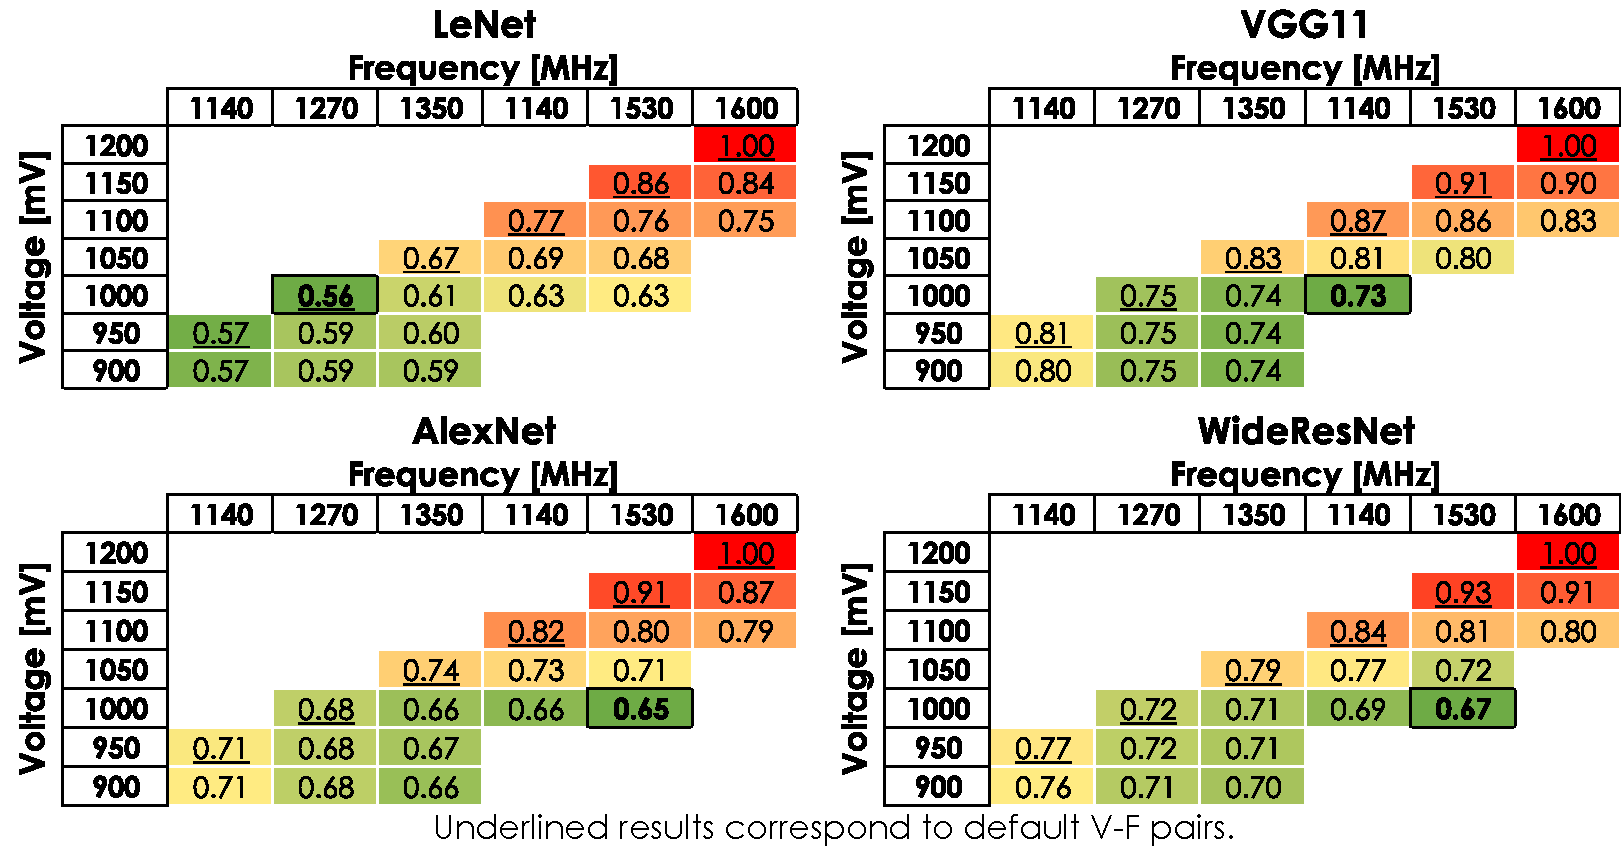
\includegraphics[width=0.8\textwidth]{Figures/Application To Deep Learning/CNN_EDP.pdf}
        \caption{Core domain - CNN models - Obtained Energy-Delay Product (EDP) for training + inference.}
    \label{fig:CNN_EDP_training_inf}
\end{figure}

\begin{table}[t]
\centering
\caption{Evaluation of performance, energy, and EDP when applying non-conventional DVFS in the training of neural networks.}
\label{tab:trainingMetricsResults}
\resizebox{\columnwidth}{!}{%
\begin{tabular}{llcccc}
&  &  \multicolumn{4}{c}{\textbf{Improvement {\it vs} default V-F}} \\ 
\cline{3-6} 
\bf Metric &  \bf Selected configuration &    \textbf{AlexNet} &  \textbf{LeNet} &  \textbf{VGG11} &  \textbf{WideResNet} \\ \hline
\textbf{Energy}        & At highest frequency & 24\% & 20\% & 22\% & 23\% \\
\textbf{}              & At best EDP          & 38\% & 38\% & 33\% & 38\% \\\hline
\textbf{Training time} & At highest frequency & 1\%  & 2\%  & 0\%  & 6\%  \\
\textbf{}              & At best EDP          & 3\%  & -3\% & -2\% & 0\% \\\hline
\textbf{EDP}           & At highest frequency & 21\% & 22\% & 22\% & 23\% \\
\textbf{}              & At best EDP          & 38\% & 41\% & 32\% & 36\% \\ \hline

&  &\multicolumn{4}{c}{\textbf{Improvement {\it vs} F scaling with default V-F pairs}} \\ \hline
\textbf{Energy}        &At best EDP&  -2\% & 0\% & -1\% & -2\% \\\hline
\textbf{Training time} &At best EDP&  8\%  & 0\%  & 6\%  & 10\%  \\\hline
\textbf{EDP}           &At best EDP&  3\% & 0\% & 3\% & 6\% \\ \hline
\multicolumn{6}{c}{a positive value indicates an improvement vs the default V-F configuration of the GPU.} \\
\end{tabular}%
}
\end{table}



\subsubsection{Inference}


\subsection{Optimization algorithm adaptation to CNN training}

As described, the optimization mechanism is comprised of two phases. This section presents how each of them was adapted to the training of \acrshort{cnn}s.


\subsubsection{Pre-run Optimization}

\subsubsection{Online Monitoring Optimization}



\subsection{Energy-efficiency Optimization}



\section{Summary}
% % ----------------------------------------------------------------------
% \subsection{Figures}
% \label{subsection:figures}

% Insert your section material and possibly a few figures...

% Make sure all figures presented are referenced in the text!


% % ----------------------------------------------------------------------
% \subsubsection{Images}
% \label{subsection:images}

% \begin{figure}[!htb]
%   \centering
%   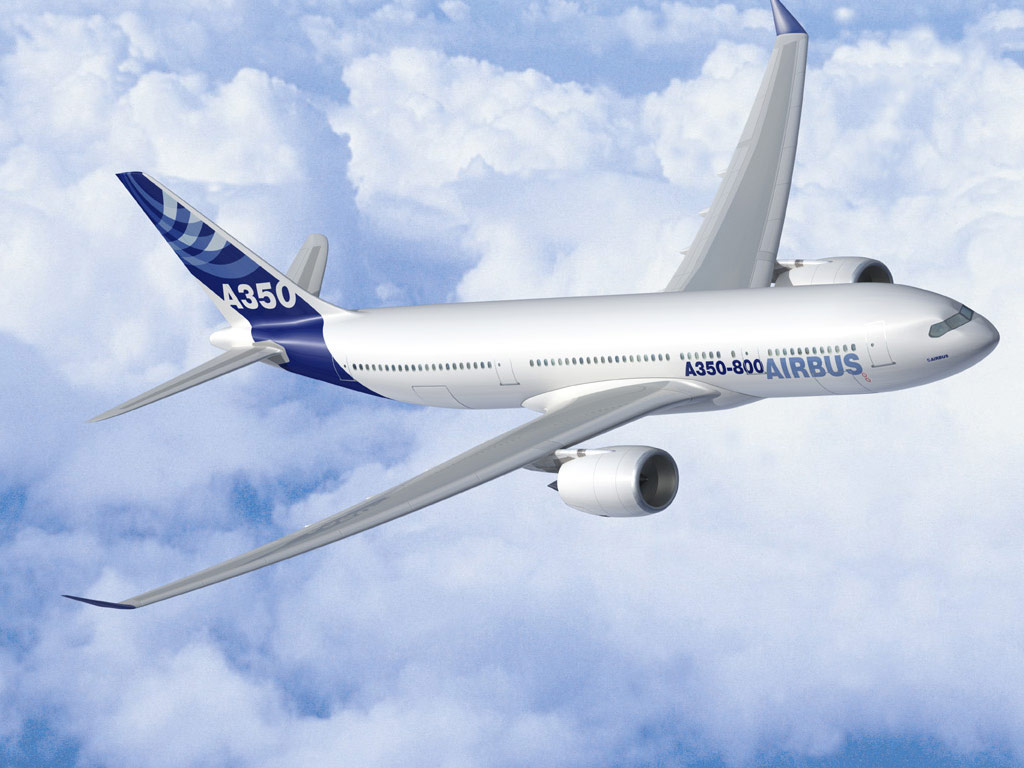
\includegraphics[width=0.25\textwidth]{Figures/Airbus_A350.jpg}
%   \caption[Caption for figure in TOC.]{Caption for figure.}
%   \label{fig:airbus1}
% \end{figure}

% \begin{figure}[!htb]
%   \begin{subfigmatrix}{2}
%     \subfigure[Airbus A320]{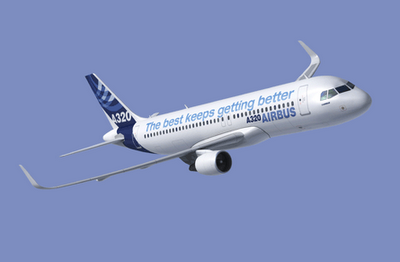
\includegraphics[width=0.49\linewidth]{Figures/Airbus_A320_sharklets.png}}
%     \subfigure[Bombardier CRJ200]{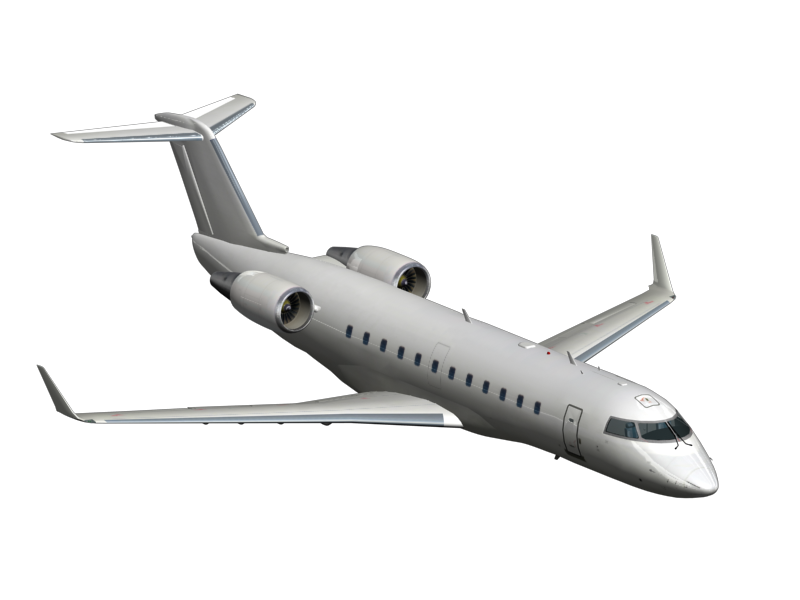
\includegraphics[width=0.49\linewidth]{Figures/Bombardier_CRJ200.png}}
%   \end{subfigmatrix}
%   \caption{Some aircrafts.}
%   \label{fig:aircrafts}
% \end{figure}

% Make reference to Figures \ref{fig:airbus1} and \ref{fig:aircrafts}.

% By default, the supported file types are {\it .png,.pdf,.jpg,.mps,.jpeg,.PNG,.PDF,.JPG,.JPEG}.

% See \url{http://mactex-wiki.tug.org/wiki/index.php/Graphics_inclusion} for adding support to other extensions.


% % ----------------------------------------------------------------------
% \subsubsection{Drawings}
% \label{subsection:drawings}

% Insert your subsection material and for instance a few drawings...

% The schematic illustrated in Fig.~\ref{fig:algorithm} can represent some sort of algorithm.

% \begin{figure}[!htb]
%   \centering
%   \scriptsize
% %  \footnotesize 
% %  \small
%   \setlength{\unitlength}{0.9cm}
%   \begin{picture}(8.5,6)
%     \linethickness{0.3mm}

%     \put(3,6){\vector(0,-1){1}}
%     \put(3.5,5.4){$\bf \alpha$}
%     \put(3,4.5){\oval(6,1){}}
%     %\put(0,4){\framebox(6,1){}}
%     \put(0.3,4.4){Grid Generation: \quad ${\bf x} = {\bf x}\left({\bf \alpha}\right)$}

%     \put(3,4){\vector(0,-1){1}}
%     \put(3.5,3.4){$\bf x$}
%     \put(3,2.5){\oval(6,1){}}
%     %\put(0,2){\framebox(6,1){}}
%     \put(0.3,2.4){Flow Solver: \quad ${\cal R}\left({\bf x},{\bf q}\left({\bf x}\right)\right) = 0$}

%     \put(6.0,2.5){\vector(1,0){1}}
%     \put(6.4,3){$Y_1$}

%     \put(3,2){\vector(0,-1){1}}
%     \put(3.5,1.4){$\bf q$}
%     \put(3,0.5){\oval(6,1){}}
%     %\put(0,0){\framebox(6,1){}}
%     \put(0.3,0.4){Structural Solver: \quad ${\cal M}\left({\bf x},{\bf q}\left({\bf x}\right)\right) = 0$}

%     \put(6.0,0.5){\vector(1,0){1}}
%     \put(6.4,1){$Y_2$}

%     %\put(7.8,2.5){\oval(1.6,5){}}
%     \put(7.0,0){\framebox(1.6,5){}}
%     \put(7.1,2.5){Optimizer}
%     \put(7.8,5){\line(0,1){1}}
%     \put(7.8,6){\line(-1,0){4.8}}
%   \end{picture}
%   \caption{Schematic of some algorithm.}
%   \label{fig:algorithm}
% \end{figure}


% % ----------------------------------------------------------------------
% \subsection{Equations}
% \label{subsection:equations}

% Equations can be inserted in different ways.

% The simplest way is in a separate line like this

% \begin{equation}
%   \frac{{\rm d} q_{ijk}}{{\rm d} t} + {\cal R}_{ijk}({\bf q}) = 0 \,.
% \label{eq:ode}
% \end{equation}

% If the equation is to be embedded in the text. One can do it like this ${\partial {\cal R}}/{\partial {\bf q}}=0$.

% It may also be split in different lines like this

% \begin{eqnarray}
%   {\rm Minimize}   && Y({\bf \alpha},{\bf q}({\bf \alpha}))            \nonumber           \\
%   {\rm w.r.t.}     && {\bf \alpha} \,,                                 \label{eq:minimize} \\
%   {\rm subject~to} && {\cal R}({\bf \alpha},{\bf q}({\bf \alpha})) = 0 \nonumber           \\
%                   &&       C ({\bf \alpha},{\bf q}({\bf \alpha})) = 0 \,. \nonumber
% \end{eqnarray}

% It is also possible to use subequations. Equations~\ref{eq:continuity}, \ref{eq:momentum} and \ref{eq:energy} form the Naver--Stokes equations~\ref{eq:NavierStokes}.

% \begin{subequations}
%     \begin{equation}
%     \frac{\partial \rho}{\partial t} + \frac{\partial}{\partial x_j}\left( \rho u_j \right) = 0 \,,
%     \label{eq:continuity}
%     \end{equation}
%     \begin{equation}
%     \frac{\partial}{\partial t}\left( \rho u_i \right) + \frac{\partial}{\partial x_j} \left( \rho u_i u_j + p \delta_{ij} - \tau_{ji} \right) = 0, \quad i=1,2,3 \,,
%     \label{eq:momentum}
%     \end{equation}
%     \begin{equation}
%         \frac{\partial}{\partial t}\left( \rho E \right) + \frac{\partial}{\partial x_j} \left( \rho E u_j + p u_j - u_i \tau_{ij} + q_j \right) = 0 \,.
%     \label{eq:energy}
%     \end{equation}
% \label{eq:NavierStokes}%
% \end{subequations}


% % ----------------------------------------------------------------------
% \subsection{Tables}
% \label{section:tables}

% Insert your subsection material and for instance a few tables...

% Make sure all tables presented are referenced in the text!

% Follow some guidelines when making tables:

% \begin{itemize}
%   \item Avoid vertical lines
%   \item Avoid “boxing up” cells, usually 3 horizontal lines are enough: above, below, and after heading
%   \item Avoid double horizontal lines
%   \item Add enough space between rows
% \end{itemize}

% \begin{table}[!htb]
%   \renewcommand{\arraystretch}{1.2} % more space between rows
%   \centering
%   \begin{tabular}{lccc}
%     \toprule
%     Model           & $C_L$ & $C_D$ & $C_{M y}$ \\
%     \midrule
%     Euler           & 0.083 & 0.021 & -0.110    \\
%     Navier--Stokes  & 0.078 & 0.023 & -0.101    \\
%     \bottomrule
%   \end{tabular}
%   \caption[Table caption shown in TOC.]{Table caption.}
%   \label{tab:aeroCoeff}
% \end{table}

% Make reference to Table \ref{tab:aeroCoeff}.

% Tables \ref{tab:memory} and \ref{tab:multipleColumns} are examples of tables with merging columns:

% \begin{table}[!htb]
%   \renewcommand{\arraystretch}{1.2} % more space between rows
%   \centering
%   \begin{tabular}[]{lrr}
%     \toprule
%                 & \multicolumn{2}{c}{\underline{Virtual memory [MB]}} \\
%                 & Euler       & Navier--Stokes \\
%     \midrule
%       Wing only &  1,000      &    2,000       \\
%       Aircraft  &  5,000      &   10,000       \\
%       (ratio)   & $5.0\times$ & $5.0\times$    \\
%     \bottomrule
%   \end{tabular}
%   \caption{Memory usage comparison (in MB).}
%   \label{tab:memory}
% \end{table}

% \begin{table}[!htb]
%   \centering
%   \renewcommand{\arraystretch}{1.2} % more space between rows
%   \begin{tabular}{@{}rrrrcrrr@{}} % remove space to the vertical edges @{}...@{}
%     \toprule
%       & \multicolumn{3}{c}{$w = 2$} & \phantom{abc} & \multicolumn{3}{c}{$w = 4$} \\
%     \cmidrule{2-4}
%     \cmidrule{6-8}
%       & $t=0$ & $t=1$ & $t=2$ && $t=0$ & $t=1$ & $t=2$ \\
%     \midrule
%       $dir=1$
%       \\
%       $c$ &  0.07 &  0.16 &  0.29 &&  0.36 &  0.71 &   3.18 \\
%       $c$ & -0.86 & 50.04 &  5.93 && -9.07 & 29.09 &  46.21 \\
%       $c$ & 14.27 &-50.96 &-14.27 && 12.22 &-63.54 &-381.09 \\
%       $dir=0$
%       \\
%       $c$ &  0.03 &  1.24 &  0.21 &&  0.35 & -0.27 &  2.14 \\
%       $c$ &-17.90 &-37.11 &  8.85 &&-30.73 & -9.59 & -3.00 \\
%       $c$ &105.55 & 23.11 &-94.73 &&100.24 & 41.27 &-25.73 \\
%     \bottomrule
%   \end{tabular}
%   \caption{Another table caption.}
%   \label{tab:multipleColumns}
% \end{table}

% An example with merging rows can be seen in Tab.\ref{tab:multipleRows}.

% \begin{table}[!htb]
%   \renewcommand{\arraystretch}{1.2} % more space between rows
%   \centering
%   \begin{tabular}{ccccc}
%     \toprule
%       \multirow{2}{*}{ABC} & \multicolumn{4}{c}{header} \\
%       \cmidrule{2-5} & 1.1 & 2.2 & 3.3 & 4.4 \\
%     \midrule
%       \multirow{2}{*}{IJK} & \multicolumn{2}{c}{\multirow{2}{*}{group}} & 0.5 & 0.6 \\
%       \cmidrule{4-5}       & \multicolumn{2}{c}{}                       & 0.7 & 1.2 \\
%     \bottomrule
%   \end{tabular}
%   \caption{Yet another table caption.}
%   \label{tab:multipleRows}
% \end{table}

% If the table has too many columns, it can be scaled to fit the text widht, as in Tab.\ref{tab:scale}.
% \begin{table}[!htb]
%   \renewcommand{\arraystretch}{1.2} % more space between rows
%   \centering
%   \resizebox*{\textwidth}{!}{%
%     \begin{tabular}[]{lcccccccccc}
%       \toprule
%         Variable &  a  &  b  &  c  &  d  &  e  &  f  &  g  &  h  &  i  &  j  \\
%       \midrule
%         Test 1   &  10,000 &  20,000 &  30,000 &  40,000 &  50,000 &  60,000 &  70,000 &  80,000 &  90,000 & 100,000 \\
%         Test 2   &  20,000 &  40,000 &  60,000 &  80,000 & 100,000 & 120,000 & 140,000 & 160,000 & 180,000 & 200,000 \\
%       \bottomrule
%     \end{tabular}
%   }%
%   \caption{Very wide table.}
%   \label{tab:scale}%
% \end{table}


% % ----------------------------------------------------------------------
% \subsection{Mixing}
% \label{section:mixing}

% If necessary, a figure and a table can be put side-by-side as in Fig.\ref{fig:side_by_side}

% \begin{figure}[!htb]
%   \begin{minipage}[b]{0.60\linewidth}
%     \centering
%     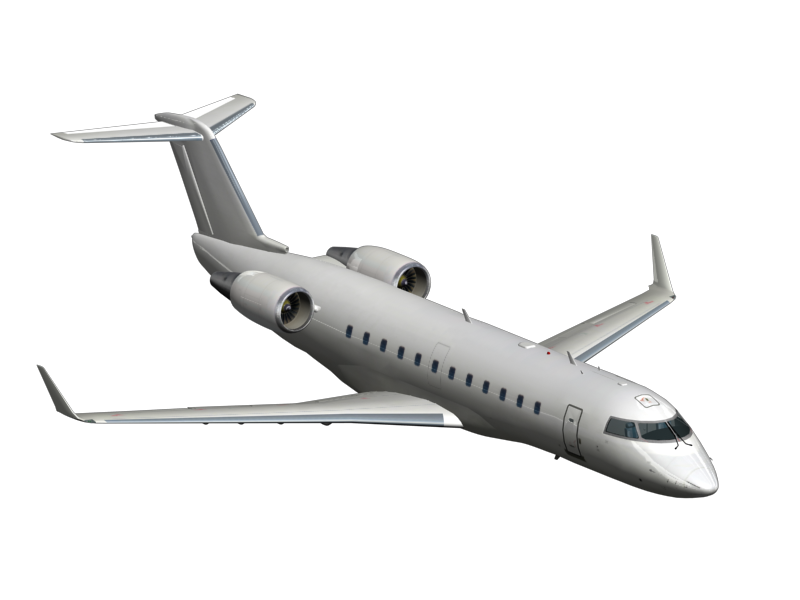
\includegraphics[width=\linewidth]{Figures/Bombardier_CRJ200}
%   \end{minipage}%
%   \begin{minipage}[b]{0.30\linewidth}
%     \centering
%     \begin{tabular}[b]{lll}
%       \toprule
%         \multicolumn{3}{c}{Legend} \\
%       \midrule
%         A & B & C \\
%         0 & 0 & 0 \\
%         0 & 1 & 0 \\
%         1 & 0 & 0 \\
%         1 & 1 & 1 \\
%       \bottomrule
%     \end{tabular}
%     \vspace{5em}
%   \end{minipage}
% \caption{Figure and table side-by-side.}
% \label{fig:side_by_side}
% \end{figure}

